\chapter[Referencial Teórico]{Referencial Teórico}

\section{Linguagens Formais}
\label{sec:languages}

Na maior parte das linguagens naturais (ex. português, inglês, etc),
letras, palavras e sentenças são entidades distintas.
Também é verdade que existem agrupamentos, isto é, conjuntos de letras
formam palavras e conjuntos de palavras formam sentenças. Contudo, 
nem todos esses conjuntos são válidos \cite{cohen1986}.

Esse tipo de relação também é válido para linguagens em computadores.
Por exemplo, na linguagem de programação \textit{C}, conjuntos de caracteres formam comandos
e um conjunto desses comandos formam programas. Estes também podem ser válidos ou não.

O estudo de linguagens formais busca entender como funcionam as linguagens de maneira unificada 
e utilizando regras bem definidas. Isto implica em definir sem ambiguidades, o que é uma linguagem e
como validar uma linguagem além de propor algoritmos específicos para realizar esta análise. 
O formalismo também pressupõe que esta área não busca compreender a comunicação ou a interpretação 
subjetiva de textos.

Para definirmos uma linguagem de maneira formal, é necessário definir algumas abstrações.
Uma destas são os Símbolos que são as unidades fundamentais de uma linguagem. Um conjunto
de símbolos válidos é o chamado alfabeto. Uma sequência de símbolos é chamado \textit{string} 
e um conjunto específico dessas \textit{strings} quando consideradas bem formadas definem uma linguagem. 

Deste modo, podemos definir uma linguagem 
como um conjunto contável de \textit{strings} que usa símbolos de um alfabeto especificado. 
Usando essa definição o português é definido como o conjunto de todos os textos 
válidos em português \cite{cohen1986}.

Entretanto, esse conjunto é infinito e portanto para definir esta linguagem de maneira precisa
é necessário utilizar as regras gramaticais e definir a linguagem de maneira
generativa utilizando uma descrição finita de regras. 

Utilizando essa estratégia, frases em português que estão semanticamente erradas porém gramaticalmente
corretas são consideradas válidas. Por exemplo, 
"Os dinossauros tem sua ética definida na tangente do verbo", são válidas para
a linguagem, visto que linguagens formais não estudam o significado dos textos.

Para compor novas linguagens, a definição permite construir linguagens complexas a partir de
outras linguagens mais simples. Para tal, é possível fazer algumas operações em linguagens
e gerar outras mais abrangentes.

Por exemplo, dado duas linguagens: L definida por duas palavras \textbf{aa} e \textbf{bb} e
D o conjunto de dígitos de \textbf{0} a \textbf{9}. Podemos definir as operações nessas 
linguagens da seguinte maneira:

\begin{itemize} 
    \item A União entre linguagens é similar à operação em conjuntos, isto é a união de L e D significa
    um novo conjunto composto pelas palavras da linguagem L mais os dígitos da linguagem D, isto é,
    o conjunto com \textbf{aa}, \textbf{bb} e os dígitos de \textbf{0} a \textbf{9}.
    \item A Concatenação de linguagens é uma operação similar ao produto cartesiano em conjuntos,
    isto é, o novo conjunto é formado utilizando todas as palavras de L e combinando com as
    palavras da linguagem D. No caso as \textit{strings} da nova linguagem possuem três caracteres
    onde os dois primeiros pertencem ao alfabeto de L e o terceiro ao alfabeto de D, por exemplo
    \textit{aa4}.
    \item A operação \textit{kleene closure} em uma linguagem consiste no conjunto de \textit{strings} criadas 
    concatenando a linguagem zero ou mais vezes, por exemplo aplicar esta operação na 
    linguagem L significa construir uma nova linguagem onde é válido \textit{strings} compostas por
    \textbf{aa} e \textbf{bb} de maneira concatenada, por exemplo \textit{aabbaaaa}.
\end{itemize}

Existem outras operações mais complexas baseadas em recursão que serão discutidas adiante.

Todo esse formalismo permitiu o desenvolvimento de técnicas para interpretar linguagens por meio de computadores.
Um exemplo disso é a área de compiladores. Duas partes fundamentais serão exploradas nas próximas
seções, análise léxica e análise sintática, estas utilizam o formalismo para construir sistemas capazes 
de reconhecer linguagens e transformar em representações para o uso do computador.

\section{Análise Léxica}

O objetivo da análise léxica é ler uma sequência de caracteres como entrada, agrupar essa entrada em 
\textit{strings} chamadas lexemas e então produzir como saída um conjunto de 
tokens para cada lexema construído. O analisador léxico também pode limpar espaços 
em brancos, comentários e outros caracteres que podem ser ignorados da entrada \cite{aho2006}.

Um token é uma estrutura que possui um tipo, uma referência ao lexema e podem ter atributos como número de linha 
e/ou coluna.
O tipo do token é um símbolo abstrato que representa uma unidade léxica, isto é, uma  palavra chave ou
uma sequência de caracteres que definem um identificador e o valor é algum atributo associado àquele token.

Podemos fazer uma analogia com o português, os lexemas são as palavras da língua e os tokens são
a classe gramatical.

Outro conceito importante é o padrão de formação, este é uma descrição da forma em que lexemas de
um token podem ocorrer na entrada. Portanto, para construir um lexema é necessário 
encontrar uma sequência de caracteres na entrada que corresponde a algum padrão predefinido.
Por exemplo, um token que representa números inteiros pode corresponder a um padrão que agrupa
qualquer sequência de dígitos em um único lexema.

Para construir um analisador léxico é necessário portanto especificar os padrões de formação para cada token. 
Isto é, descrever como devem ser os lexemas para cada token. Esse padrão é comumente especificado 
utilizando expressões regulares.

\subsection{Expressões Regulares}

Expressões regulares são uma notação utilizada para descrever um tipo específico de linguagem, as linguagens regulares.
Linguagens regulares usam as operações descritas em \ref{sec:languages} e associam uma sintaxe
específica a cada uma destas três operações. As implementações encontradas na maioria das linguagens de programação
são baseadas na sintaxe proposta pelo Perl e em alguns casos adicionam extensões não regulares à
linguagem.

Essas expressões são construídas recursivamente a partir de expressões menores. 
A unidade básica dessa expressão são os símbolos de um alfabeto. Por exemplo,
se o caractere \textit{a} pertence a algum alfabeto então \textbf{a} é 
uma expressão regular que representa uma linguagem definida apenas pela palavra \textit{a}.

Supondo que \textbf{r} e \textbf{s} são expressões regulares. Então, as operações básicas 
são representadas pela seguinte notação:

\begin{itemize}
    \item (\textbf{r})|(\textbf{s}) expressão regular que denota união entre as linguagens L(\textbf{r}) e 
    L(\textbf{s}).
    \item (\textbf{r})(\textbf{s}) expressão regular que denota concatenação entre as linguagens L(\textbf{r}) e 
    L(\textbf{s}).
    \item (\textbf{r})* expressão regular que representa a operação \textit{kleene closure} na linguagem L(\textbf{r}).
    \item (\textbf{r}) expressão regular que representa a linguagem L(\textbf{r}). Os parentêses não mudam
    a linguagem representada, e servem apenas para desambiguar expressões. Por exemplo, 
    na expressão ((\textbf{r})|(\textbf{s}))* os últimos parentêses deixam explícito para qual expressão 
    o operador \textit{kleene} está sendo aplicado.
\end{itemize}

Por exemplo, dado que \textit{l} representa todas as letras e o \textit{underscore} 
aceitas pela linguagem C e que \textit{d} representa todos as os dígitos aceitos 
pela linguagem C, então os identificadores da linguagem C podem ser descritos utilizando 
a expressão regular:

\begin{center}
l(l|d)*
\end{center}
Isto significa que identificadores em C sempre começam com uma letra ou \textit{underscore} 
e podem ter zero ou mais letras, \textit{underscores} e dígitos subsequentes.

\section{Análise Sintática}
\label{sec:sintatic}

A análise léxica lê vários caracteres da entrada e os agrupa em uma sequência de tokens. Essa sequência de
tokens não necessariamente define uma entrada válida e portanto é importante ter alguma maneira de
validar a sintaxe dessa entrada.

A análise sintática é o processo onde é verificada a sintaxe da entrada. 
Para fazer essa verificação são utilizadas regras precisas que especificam 
uma estrutura sintática válida \cite{aho2006}.

A especificação dessas regras pode ser feita utilizando uma notação chamada gramática 
livre de contexto, nela as regras de sintaxe são definidas de 
maneira precisa e fácil de entender.

Mais formalmente, uma gramática livre de contexto consiste em quatro partes. Sendo elas
o conjunto dos terminais, o conjunto dos não terminais, o símbolo inicial e as produções.

\begin{description}
    \item[Terminais:] São os símbolos básicos que formam a sequência de 
    caracteres da entrada. O analisador léxico retorna tokens que possuem terminais. 
    \item [Não Terminais:] Chamados de variáveis sintáticas denotam conjuntos 
    de sequências de caracteres. Também impõe uma estrutura hierárquica na linguagem.
    \item[Símbolo Inicial:] Diferencia um não terminal para ser considerado 
    como inicial na interpretação da gramática. Corresponde à raiz da árvore sintática
    resultante.
    \item[Produção:] Declara a maneira como os terminais e não terminais 
    podem ser combinados para formar uma entrada válida. É dividido em três partes,
    como em a : $\beta$, o lado esquerdo que possui um não terminal, e o lado direito 
    ou corpo da produção que, consiste de zero ou mais terminais e/ou não terminais e especifica
    a forma de construir uma sequência de caracteres para o não terminal referente a seu lado esquerdo.
\end{description}

A notação utilizada é uma \textit{Backus Normal Form} extendida baseada na 
biblioteca Lark\footnote{\url{https://github.com/lark-parser/lark}}. Nesta notação os não 
terminais são sempre escritos em caixa baixa e os terminais podem ser escritos de duas 
maneiras, literais simples utilizando aspas duplas ou terminais complexos escritos em caixa alta \cite{lark}.

A gramática exemplificada no Código \ref{lst:grammar} define uma linguagem capaz de representar 
expressões aritméticas simples. Os não terminais são: expr, term e factor. 
Os terminais são: "+", "-", "*", "/", "(", ")" e ID (representa um identifador que é definido usando
uma expressão regular). Por fim, o símbolo inicial é expr.

\begin{lstlisting}[caption=Exemplo de gramática livre do contexto que descreve expressões
    aritméticas como (20 + 1) * 2.,label={lst:grammar}]
expr : expr "+" term 
     | expr "-" term
     | term

term : term "*" factor
     | term "/" factor
     | factor

factor : "(" expr ")"
       | ID
\end{lstlisting}

Para a construção de um analisador sintático (\textit{parser}) é importante entender o conceito de derivação. 
A partir do símbolo inicial são feitos passos de reescrita onde um não terminal é substituído pelo
corpo da sua produção. 

Por exemplo, considere a primeira produção da gramática na linha 1 do Código \ref{lst:grammar}. 
Essa linha pode ser lida da seguinte maneira "expr \textbf{deriva} expr + term". 
E isso significa que o não terminal expr pode ser substituído pela produção expr + term. 

Por exemplo, a notação utilizada para representar essa substituição é.
\begin{center}
expr $\Rightarrow$ 40 + 2
\end{center}
Além disso, essas substituições podem ser aplicadas de forma sequencial. Por exemplo,
\begin{center}
    expr $\Rightarrow$ expr + term $\Rightarrow$ term + factor $\Rightarrow$ factor + 2 $\Rightarrow$ 40 + 2
\end{center}
Essa sequência de substituições é denominada derivação e possui papel fundamental para entender
como construir um analisador sintático \cite{aho2006}. 

Outro conceito importante para a construção de um analisador sintático são
as \textit{parse trees} que representam uma derivação utilizando a estrutura de dados árvore, 
pode-se dizer que essa árvore também representa a entrada.

\begin{figure}[h]
	\centering
	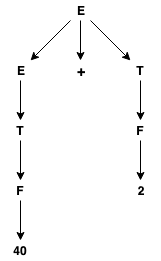
\includegraphics[keepaspectratio=true,scale=1]{figuras/parsetree.png}
	\caption{Exemplo de Parse Tree.}
	\label{fig:parsetree}
\end{figure}

Utilizando a gramática especificada no Código \ref{lst:grammar}, porém com uma pequena alteração
onde os não terminais são representados apenas pelas suas primeiras letras, teríamos a Fig. \ref{fig:parsetree}. 
Essa árvore equivale à derivação a seguir:

\begin{center}
    E $\Rightarrow$ E + T $\Rightarrow$ T + T $\Rightarrow$ F + T $\Rightarrow$ 40 + T $\Rightarrow$ 40 + F $\Rightarrow$ 40 + 2
\end{center}

Existem três tipos genéricos de \textit{parsers} para gramáticas livre de contexto: 
universal, \textit{top-down} e \textit{bottom-up}. Os métodos de \textit{parsing}
universais podem analisar qualquer gramática. Porém, muitas vezes sua complexidade é exponencial, por exemplo o algoritmo Earley,
um dos mais eficientes nesta categoria, tem no pior caso complexidade assintótica O($n^3$).

Normalmente os métodos mais utilizados são  \textit{top-down} ou \textit{bottom-up}. Onde, no primeiro,
a \textit{parse tree} é construída a partir do topo, da raiz até as folhas. E no segundo é o inverso,
das folhas até a raiz. 

Vale ressaltar que os analisadores mais eficientes tanto \textit{top-down} ou \textit{bottom-up}  
só funcionam para subclasses de gramáticas livres do contexto. Este documento foca nos analisadores
do tipo \textit{top-down}. Visto que, um dos os objetivos do projeto é definir um formato de fácil construção
utilizando técnicas \textit{top-down}.

\subsection{Analisadores \textit{Top-Down}}

A construção de analisadores do tipo \textit{top-down} é como o processo de
construir a \textit{parse tree} a partir do topo e isto é
equivalente a encontrar a derivação mais à esquerda para a entrada \cite{aho2006}.

Para exemplificar, considere a gramática descrita no Código \ref{lst:grammartopdown}. Esta
representa uma linguagem para expressões aritméticas parecida com a definida no 
Código \ref{lst:grammar}, porém sofreu mudanças para adequar ao processo de \textit{parsing top-down}.

Uma dessas mudanças foi retirar recursões à esquerda da gramática, pois esta leva a
problemas durante a análise \cite{aho2006}.

\begin{lstlisting}[caption=Exemplo de gramática para analisadores top-down onde o símbolo epsilon representa uma produção vazia.,label={lst:grammartopdown}]
e  : t e'

e' : "+" t e' 
   | ε

t  : f t'

t' : "*" f t' 
   | ε

f  : "(" e ")"
   | ID
\end{lstlisting}

\begin{figure}[h]
	\centering
	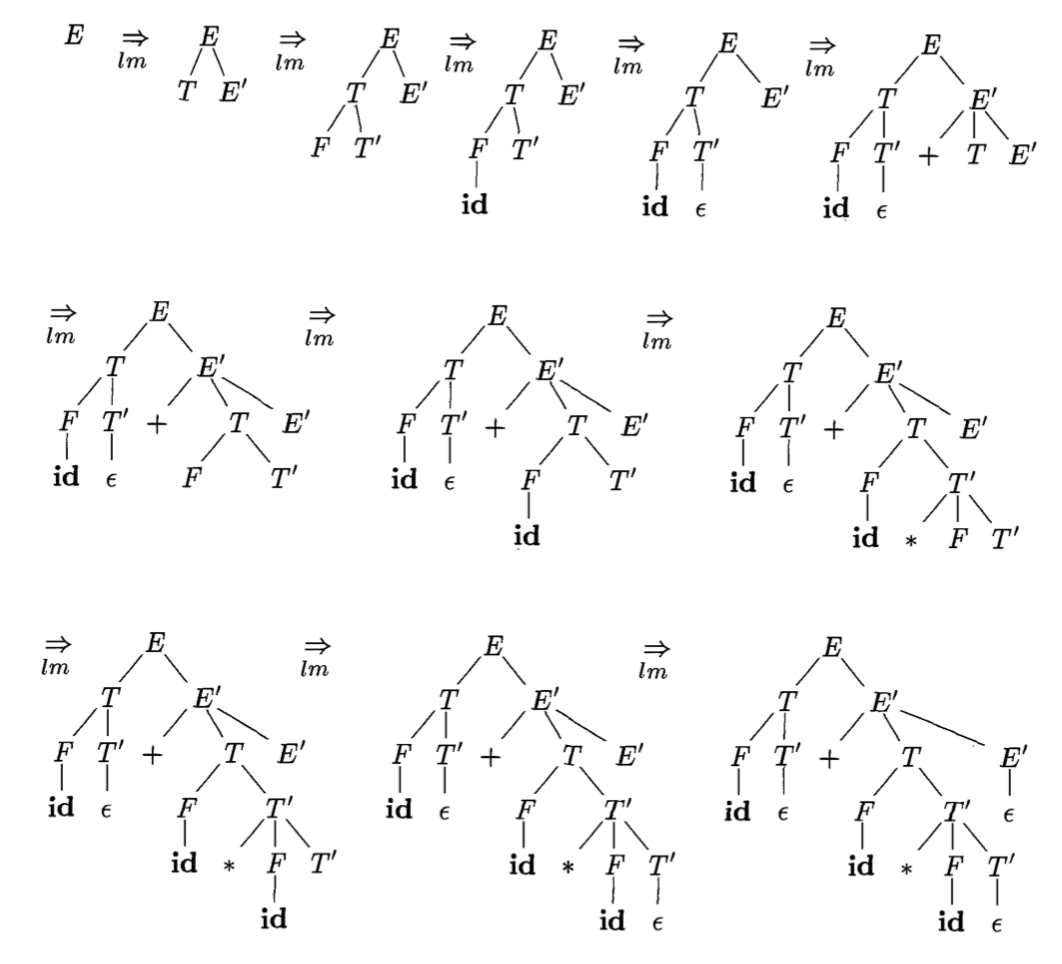
\includegraphics[keepaspectratio=true,scale=0.7]{figuras/parsetopdowntree.png}
	\caption{Exemplo de parse top-down \cite{aho2006}.}
	\label{fig:parsetopdowntree}
\end{figure}

A análise sintática a partir do topo consiste em cada etapa determinar qual produção 
aplicar para o respectivo não terminal. Depois que uma produção for escolhida
o processo resume-se a combinar os terminais no corpo da produção com os tokens da entrada.

Um exemplo de análise \textit{top-down} pode ser visualizado na Figura \ref{fig:parsetopdowntree},
onde existem várias árvores de derivação representando cada etapa do processo de análise para a 
entrada \textbf{id + id * id}. Este processo utiliza a gramática definida no Código \ref{lst:grammartopdown}.

Descida recursiva é uma maneira simples e genérica para construir um \textit{parser top-down}.
Nesse tipo de analisador existe um conjunto de procedimentos para cada não terminal \cite{aho2006}. 

A execução começa chamando recursivamente o procedimento para o símbolo inicial e então 
termina a execução com sucesso se a execução ler toda a entrada. 

Esse tipo de analisador pode necessitar de \textit{backtracking}. Isto é, ler a entrada toda
novamente repetidas vezes. Caso o caminho tomado durante o momento de escolher uma produção falhar,
é necessário reiniciar a execução usando outra produção. A necessidade de recomeçar a execução
pode elevar o tempo de execução para valores exponenciais \cite{aho2006}. 

Um exemplo de procedimento para um não terminal pode ser visto no Código \ref{lst:recursive}.

\begin{lstlisting}[caption=Exemplo de procedimento em pseudo-python para um não terminal,label={lst:recursive}]
def E(tokens):
    return [T(tokens), E_(tokens)]

def E_(tokens):
    if tokens[0] == "+":
        plus = tokens.pop(0)
        return [plus, T(tokens), E_(tokens)]
    else:
        return None

...
\end{lstlisting}


\subsection{\textit{Parser Combinators}}

Outro método para construir \textit{parsers top-down} bastante comum, 
principalmente em linguagens funcionais, são os chamados \textit{parsers combinators},
esse modelo é construído a partir de um analisador com descida recursiva \cite{hutton1996monadic}.

Essa técnica utiliza funções como \textit{parsers} e define outras funções de alta ordem que
implementam abstrações das gramáticas livres de contexto, 
isto é, sequências, escolha e repetição.

O método consiste em criar pequenos \textit{parsers} para as produções da gramática como funções. 
E utilzar as funções que representam as abstrações das gramáticas livres de contexto 
para combinar esses parsers.

Podemos definir um parser como uma função que recebe como entrada uma lista de \textit{tokens}
e tem como saída uma árvore e o restante da entrada. Um exemplo simples de parser pode ser
visto no Código \ref{lst:itemparser}, nele o primeiro item da lista é consumido apenas
se o primeiro item for um espaço em branco. Caso isso não ocorra o parser falha.

\begin{lstlisting}[caption=Exemplo de parser em pseudo-python,label={lst:itemparser}]
def whitespace(tokens):
    if not tokens or tokens[0].type != SPACE:
        raise SyntaxError
    else:
        return tokens[0], tokens[1:]
\end{lstlisting}

Um exemplo de combinador pode ser o sequenciamento, isto é aplicar um parser após o outro. 
Em gramática livre do contexto a notação para uma sequência é apenas colocar um 
item ao lado do outro na produção. O código para representar
esse combinador está no Código \ref{lst:seqcomb}.

\begin{lstlisting}[caption=Exemplo de combinador em pseudo-python,label={lst:seqcomb}]
def seq(parser1, parser2):
    def seq_parser(tokens):
        (result1, tokens) = parser1(tokens)
        (result2, tokens) = parser2(tokens)
        return ((result1, result2), tokens)
    return seq_parser
\end{lstlisting}

\textit{Parser combinators} implementam gramáticas a partir da composição de funções deste tipo
com funções primitivas.

\subsection{\textit{Parser} LL(1)}

Existe uma classe de \textit{parsers} chamada preditiva que evitam a necessidade de \textit{backtracking}. 
Ela consegue determinar a próxima produção a ser executada de maneira determinística 
analisando os próximos tokens da entrada.

Um exemplo concreto são os analisadores LL(1). Neste tipo de \textit{parsing} 
o processo é parecido com a descida recursiva. Entretanto, no momento de escolher 
a produção o token atual da entrada é analisado e pode-se determinar 
a produção correta a ser escolhida. Isto evita a necessidade de fazer \textit{backtracking}.

Para construir esse tipo de \textit{parser} é necessário um algoritmo 
que permita escolher qual produção a ser executada de maneira determinística.

Este algoritmo utiliza uma \textit{predictive parsing table}. Essa tabela consiste
de linhas representando não terminais, colunas representando o símbolo de entrada e o valor
dentro da célula diz qual produção escolher durante o \textit{parsing}. 

O método para construir essa tabela necessita antes de duas operações comumente chamadas \textit{FIRST} e 
\textit{FOLLOW}.

A definição de FIRST(A), onde A é qualquer sequência de símbolos da gramática, 
é o conjunto dos terminais que iniciam as 
sequências derivadas a partir de A. 
De maneira genérica, dado uma derivação A $\Rightarrow$ ... $\Rightarrow$ cy onde c é um terminal, logo
c pertence ao conjunto FIRST(A).
Por exemplo utilizando a gramática definida no Código \ref{lst:grammartopdown}, o FIRST(F) é o conjunto com
dois terminais \textbf{(} e \textbf{ID}. Como F não deriva string vazia o FIRST(T) e FIRST(E) são iguais.

A definição de FOLLOW(A) é o conjunto de terminais x que podem aparecer imediatamente
à direita de um não terminal A. Isto é, o conjunto de terminais x em derivações na forma 
S $\Rightarrow$ ... $\Rightarrow$ wAxy onde w e y podem ser qualquer sequência de símbolos.
Por exemplo utilizando a gramática definida no Código \ref{lst:grammartopdown}, o FOLLOW(E) é composto pelo terminal \textbf{)}.

\begin{table}[h]
    \centering
	\caption{Tabela preditiva para analisador sintático LL(1)}
	\label{tbl:predictive}

    \begin{tabular}{cccccc}
        \toprule
        \multicolumn{1}{c}{\textbf{Não Terminal}} & \multicolumn{5}{c}{\textbf{Terminais}} \\
        \midrule
                       & \textbf{id} & \textbf{+} & \textbf{*} & \textbf{(} & \textbf{)}   \\
        \midrule
        \textbf{E}     &     1      &      -      &      -       &     1    &    -    \\
        \textbf{E'}    &     -      &      3      &      -       &     -    &    4    \\
        \textbf{T}     &     6      &      -      &      -       &     6    &    -    \\
        \textbf{T'}    &     -      & 9           &      8       &     -    &    9    \\
        \textbf{F}     &     12     &      -      &      -       &     11   &    -    \\
        \bottomrule
    \end{tabular}
\end{table}

Um exemplo de tabela preditiva pode ser visto na Tabela \ref{tbl:predictive}, os números referenciam as linhas 
do Código \ref{lst:grammartopdown} onde estão as produções.

Neste capítulo foi discutida a fundamentação teórica necessária para entender como um computador pode
interpretar uma linguagem. O próximo capítulo discute vários formatos utilizados para serialização de dados.